\section{Nombre: Tepeyóllotl}  \label{per:tepeyollotl}
\subsection{Descripción:}    
Dios jaguar, es de un tamaño ligeramente mayor al de un jaguar normal. Porta joyería fina para marcar su posición en la jerarquía divina. Usa un collar de oro con extensiones que protegen su espalda. Porta un arete de esmeralda en la oreja izquierda y un brazalete de oro en la pata izquierda. Su coraza de piedra cubre todo su cuerpo salvo por sus ojos. La coraza muestra pequeños detalles de como es Tepeyóllotl, omitiendo los detalles de su joyería y adornos, mostrando con pocas lineas detalles como su nariz y las lineas del hocico.
\\
\par
Tepeyóllotl es un personaje astuto y observador, solo necesita de observar a los demás para darse cuenta de las verdaderas intensiones de alguien pero se guardará sus descubrimientos para él mismo a no ser que pueda obtener alguna ventaja por comunicárselo a alguien. Como cualquier felino, es orgulloso, una vez herido su orgullo es difícil recuperar su amistad. 
\subsection{Status:}
	\begin{itemize}
		\item Personaje no jugable.
		\item Enemigo jefe.
	\end{itemize}
\subsection{Imagen}
Ver figura \ref{fig:TepeyollotlDiseno}
\begin{figure}
				\centering
				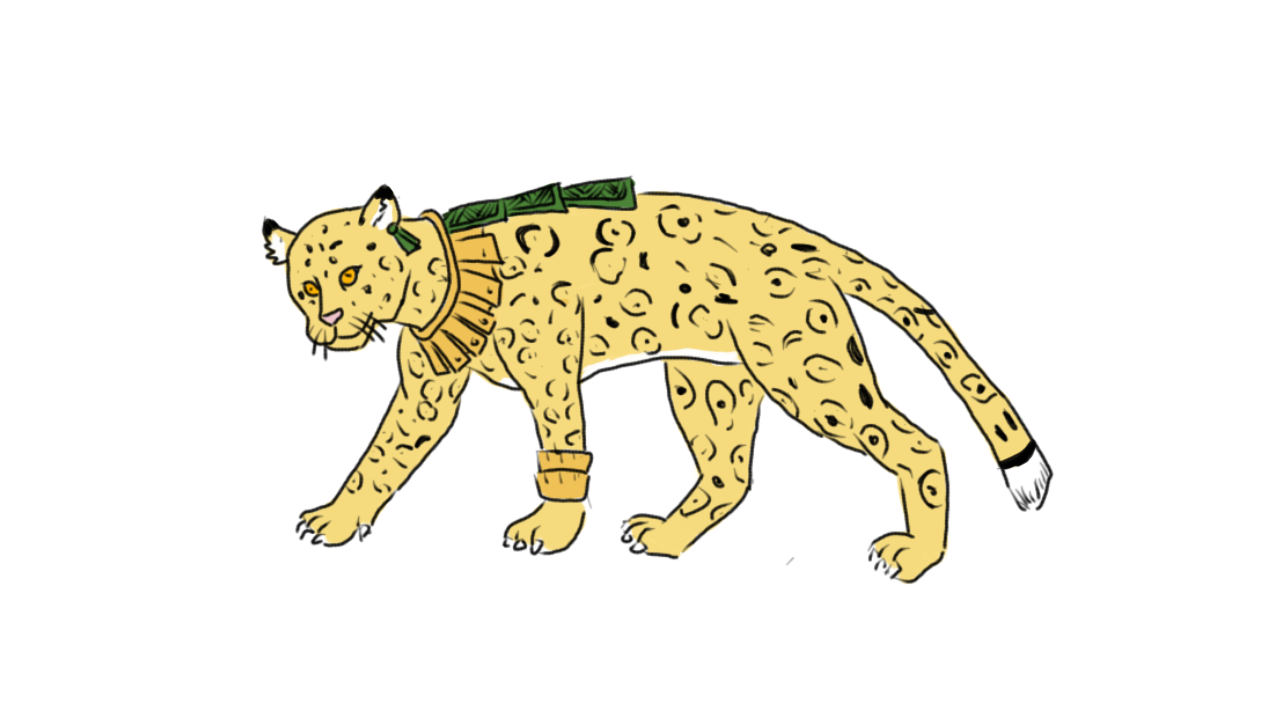
\includegraphics[height=0.3 \textheight]{Imagenes/tepeyollotl}
				\caption{Concepto de diseño de Tepeyóllotl.}
				\label{fig:TepeyollotlDiseno}
\end{figure}
\subsection{Concepto:}
\begin{itemize}
	\item \textbf{Historia antes del juego:}
	Antes de la era del quinto Sol, Tepeyóllotl gozaba de una posición medianamente favorable dentro de la jerarquía divina. Su papel se limitaba a cumplir su rol como dios de las montañas. 
	\\
	\par
	La era del quito sol trajo consigo no solo una reestructuración de la jerarquía divina sino a su vez desato un gran numero de insurrecciones por parte de diferentes Dioses que no estaban dispuestos a abandonar sus privilegios tan fácilmente. Una vez restaurado el orden, los dioses gobernantes de los trece cielos, temerosos de futuras rebeliones, designan diferentes dioses para garantizar el orden. Por ordenes de Tezcatlipoca y por su amistad con éste, Tepeyóllotl es designado como guardian del Mictlán con el objetivo de vigilar a los demás dioses e informar a Tezcatlipoca sobre cualquier irregularidad o peligro. Su rol en el Mictlán, hace que Tepeyóllotl sea el blanco de cualquier invasor que desee conquistar el Mictlán, Tepeyollotl esta consciente de esto y por tal motivo no teme seguir sus propias reglas y alejarse de su juramento como guardián del Mictlán.   
	\item \textbf{Historia durante el juego:}
	Cuando Malinalli y Xólotl llegan al Tepeme Monamictlán, Tepeyóllotl se prepara para hacerle frente a los invasores sin saber de quienes se trataban. Al descubrir que se trataba de Xólotl, Tepeyóllotl no toma enserio la amenaza. Una vez derrotado, Tepeyóllotl consigue escapar al Teyollocualóyan con la intensión de avisarle a Tezcatlipoca sobre lo que estaba ocurriendo en el Mictlán. Sin embargo, Tepeyóllotl abandona la idea de informarle a Tezcatlipoca, al percatarse del avance de Malinalli. Es entonces que Tepeyóllotl empieza a sentir algo peligroso y obscuro creciendo dentro de ella, lo que lo lleva a concluir que Malinalli tiene otros planes además de ayudar a Xólotl.
	\\
	\par
	Con cada Dios que Malinalli va derrotando, el sentimiento de incertidumbre crece en Tepeyóllotl. Es con la caída de Tlazoltéolt que Tepeyóllotl acepta que el Mictlán esta perdido, por lo que se ve en el dilema de huir del Mictlan para advertirle personalmente a Tezcatlipoca o quedarse y tratar de averiguar más sobre Malinalli con la esperanza de ponerla en contra de Xólotl. Comprendiendo los riesgos ante la posibilidad de fallo, Tepeyóllotl manda a llamar a Mictecacíhuatl para comunicarle sus pocos descubrimientos. Hecho esto, se sienta a esperar la llegada de Malinalli y Xólotl. Sus intentos por controlar a Malinalli fallan y tal como lo había previsto el mismo Tepeyóllotl: lo único que encuentra al final de la batalla es la derrota.  
	\item \textbf{Relaciones:}
	\begin{itemize}
		\item \textbf{Tezcatlipoca:} Amigo de Tepeyóllotl. Es su jefe directo en la jerarquía divina, siendo al único al que debe de rendir cuentas sin excusas (ver aparatado \ref{per:tezcatlipoca}). 
		\item \textbf{Mictecacíhuatl:} Tepeyóllotl siente una admiración sincera por ella, siendo la única con quien habla en el Mictlán. Tepeyóllotl considera que  Mictecacíhuatl debería ser la novena guardiana del  Mictlán y no Mictlantecuhtli (ver aparatado \ref{per:mictlantecutli}).
		
		\item \textbf{Mictlantecuhtli:} Desde el punto de vista de Tepeyóllotl,  Mictlantecuhtli es un líder ineficiente y de poca visión por lo que comúnmente tiene roces con él (ver aparatado \ref{per:mictecacihuatl}).
		
		\item \textbf{Xólotl:} Percibido como un niño malcriado y emberrinchado, Tepeyóllotl no tiene en buena estima a Xólotl (ver aparatado \ref{per:xolotl}).
		
		\item \textbf{Malinalli:} Considerada como el verdaero peligro para la jerarquía divina. Tepeyóllotl no se siente comodo al lado de ella pues algo le dice que la presencia de Malinalli esta ligada a la caída de todos los Dioses (ver aparatado \ref{per:malinalli}).
	\end{itemize}                     
\end{itemize}
\subsection{Encuentro:}
\begin{itemize}
	\item Su primera aparición es en la cinemática 9 (ver aparatado \ref{Cin:Cinematica09}). 
	\item El jugador se enfrenta a él como jefe del tercer nivel del juego (ver aparatado \ref{Nivel:Niv03}).
	\item El jugador se enfrenta a él como jefe del octavo nivel del juego (ver aparatado \ref{Nivel:Niv08}).
\end{itemize}

\subsection{Habilidades:}
\begin{itemize}
        \item Coraza (ver aparatado \ref{hab.coraza}).   
        \item Impacto (ver aparatado \ref{hab.impacto}).
        \item Luvia de rocas (ver aparatado \ref{hab.LLuviaRocas}). 
	  \item Rugido aturdidor (ver aparatado \ref{hab.RugAtur}). 
\end{itemize}
\subsection{Armas:}
Sin armas.
\subsection{Ítems:}
Sin ítem
\subsection{Bloques de animación}
	\begin{itemize}
		\item Con coraza
			\begin{itemize}
				\item Animación correr.
				\item Animación saltar.
				\item Animación rugir.
				\item Animación recibir daño.
				\item Animación morir.
			\end{itemize}
		\item Sin Coraza.
			\begin{itemize}
				\item Animación correr.
				\item Animación saltar.
				\item Animación rugir.
				\item Animación recibir daño.
				\item Animación morir.
			\end{itemize}
	\end{itemize}